\begin{wrapfigure}{t!}{0.5\textwidth}
	%\begin{figure}
	\centering
	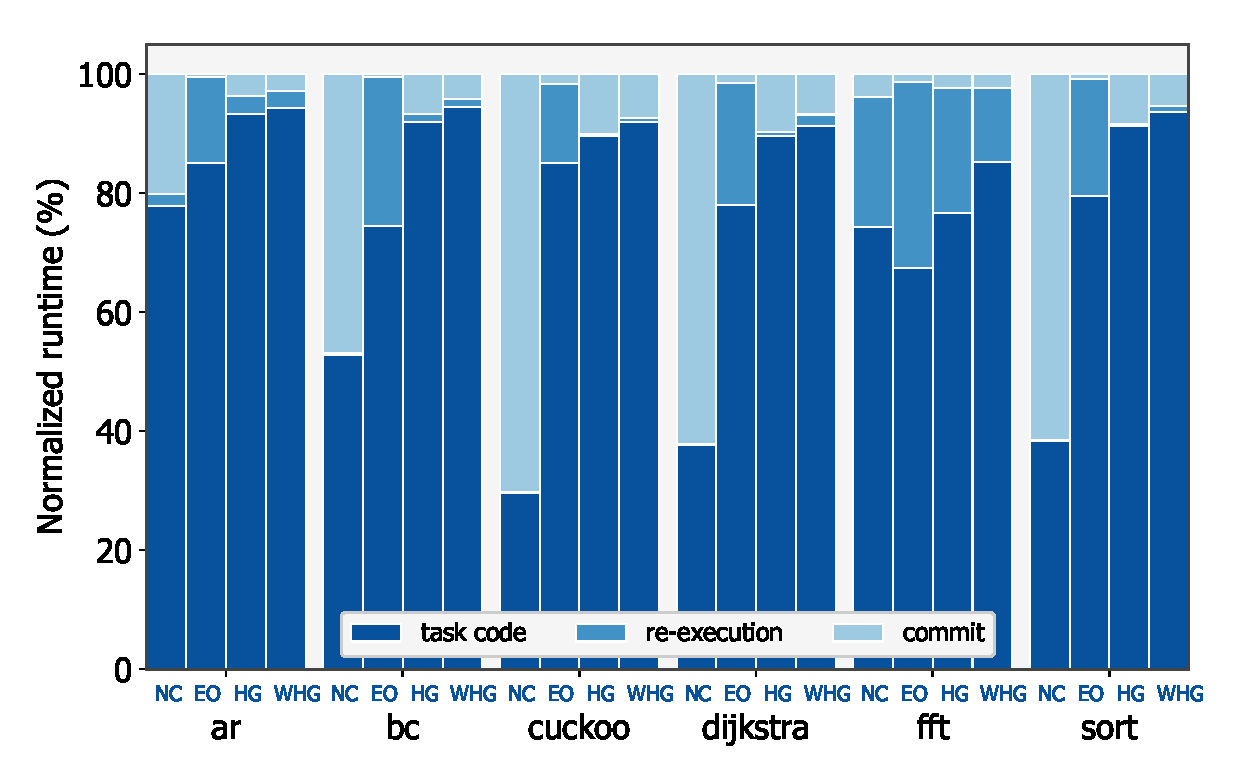
\includegraphics[width=0.5\columnwidth]{figures/coalEfficiency}
	\caption{Percent time usage for all coalescing strategies (including no-coalescing) comparing useful execution to intermittency overhead. NC: no coalescing, EB: energy-blind coalescing, EA: energy-aware coalescing, ETA: energy- and task-aware coalescing. All \sys coalescing strategies significantly reduce the overhead of (task) commits. EA and ETA perform much better than EB since they reduce re-execution penalty. \todo{rename legend entry 'user code' with 'useful task code'; rename y-axis to 'Time usage (\%)'; increase font by two more points everywhere}{Amjad}}
	\label{fig:overallOverheadBreakdown}
	%\end{figure}
\end{wrapfigure}

Our results illustrate key findings about \sys. We show through extensive qualitative and quantitative evaluation that (i) \sys \emph{provides computation progress} at the partial task level, guaranteeing execution at the worst intermittent energy conditions where state-of-the-art runtimes fail; (ii) \sys usually \emph{improves execution speed} of applications compared to state-of-the-art runtimes; (iii) \sys, through coalescing mechanism, \emph{reduces the memory protection overhead} significantly; and  that (iv) \sys is \emph{more generic to use} and allows to interact with code written for non-intermittent devices easily.

\textbf{Key Performance Indicators.} Our aim is to assess \sys as detailed as possible. For this we have characterized \sys's runtime performance (execution time), based on a set of benchmarks, considering core task adaptation mechanisms of the system: \emph{task coalescing} and \emph{task downscaling}. We also characterize \sys's overhead showing precisely what the source of \sys superior performance is, investigating task re-execution and commit penalty and memory access patterns.

We remind the reader that \sys is compared to Alpaca runtime and the benchmarks for Alpaca were hand-transformed in a time-consuming manual process from Clang (LLVM-generated code) to GCC (see Section~\ref{sec:implementation}). The manual code transformation was required as \sys was written with GCC in mind, and Alpaca cannot support any other complier than LLVM.

%Then, we need to know how many tasks \sys can coalesce within a given execution scenario. We ran a subset of applications (split by tasks manually) with continuous power supply and measured the size of tasks for each application and the amount of tasks coalesced. Result is given in Table~\ref{tab:aveVirtuTaskSize}. We see clearly that \sys manages to coalesce more tasks as individual tasks are small. As the size of individual task increases, e.g., as in the case of dft application, the number of coalesced tasks is also small. This result clearly shows that for the benefit of coalescing and for code portability, initial code should be split by \emph{as small tasks as possible}. This will help \sys to find the best possible virtual task size to minimise its runtime.

\subsection{Characterization of \sys's Overhead}
\label{sec:coala_overhead}

We start with the assessment of \sys's overhead for all benchmarks. This will lead us to the selection of the best coalescing strategy to proceed with.

\indent \textbf{Coalescing Algorithms Efficiency.} We have measured the time spent on executing (i) useful task code, (ii) wasted task code (that have to be re-executed due to uncommitted progress), and (iii) commits for all coalescing strategies (EB, EA and ETA) and all benchmarks. We compared our results to non-coalescing (NC). The experiment was performed at 15\,cm WISP-to-exciter distance and normalized per benchmark. All benchmarks were using 256\,B pages, except for \textbf{bc} which was using 32\,B pages. Those page sizes are the ones yielding acceptable performance\footnote{Detailed investigation of \sys's paging performance will be given in Section~\ref{sec:results_memory_management}.}, selected among the set mentioned in Section~\ref{sec:implementation}.

The result is presented in Figure~\ref{fig:overallOverheadBreakdown}. We clearly see that all coalescing strategies make a better use of the resources for \emph{all} benchmarks (except for EB in \textbf{bc}).
With a more thorough look, one can notice that the re-execution penalty, i.e. the time wasted running tasks whose progress could not be committed due to a power failure, is minimized by NC. This is obvious, since this strategy makes the system commit after each static task.
On the other hand, the burden on committing so frequently reflects in a degraded performance with respect to coalescing, motivating one of the needs raised by this work.
EA and ETA strategies provide the best balance between re-execution penalty and commit cost. For this reason we proceed with the investigation of \sys without considering EB coalescing.

\begin{figure}
	\centering
	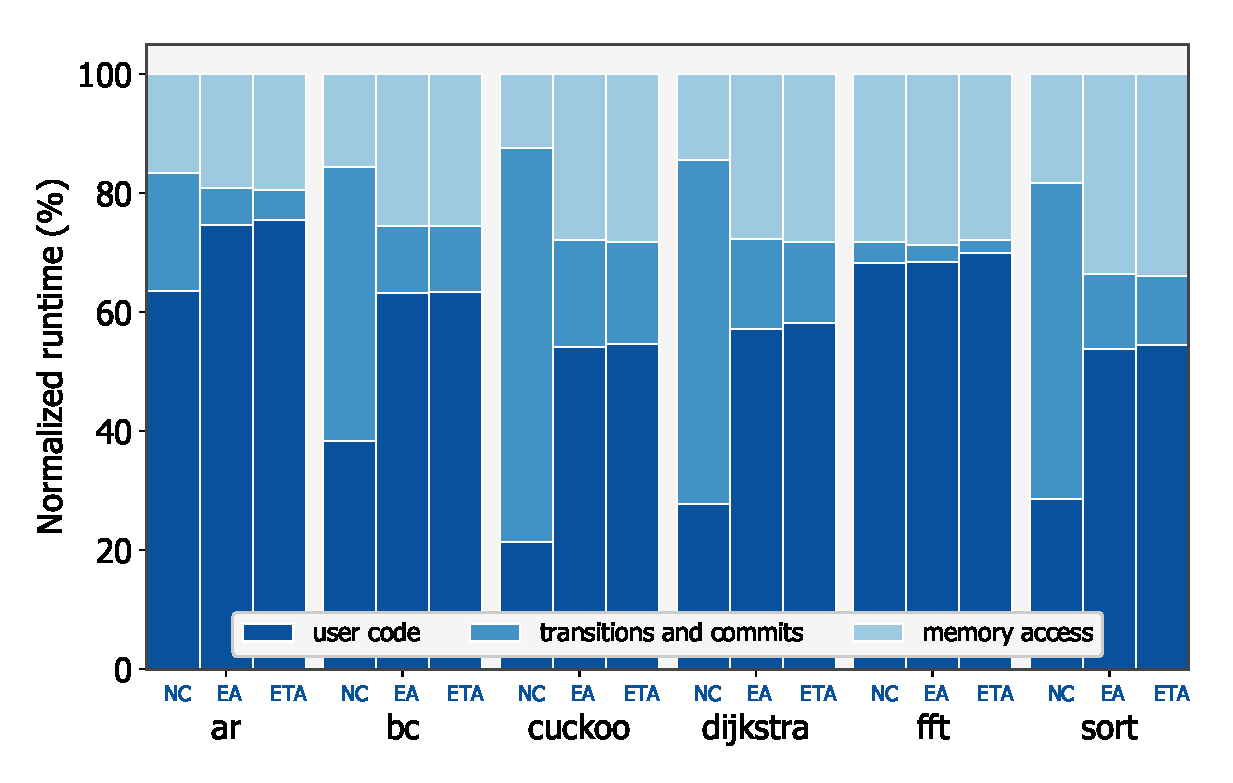
\includegraphics[width=0.49\columnwidth]{figures/overallOverhead}
	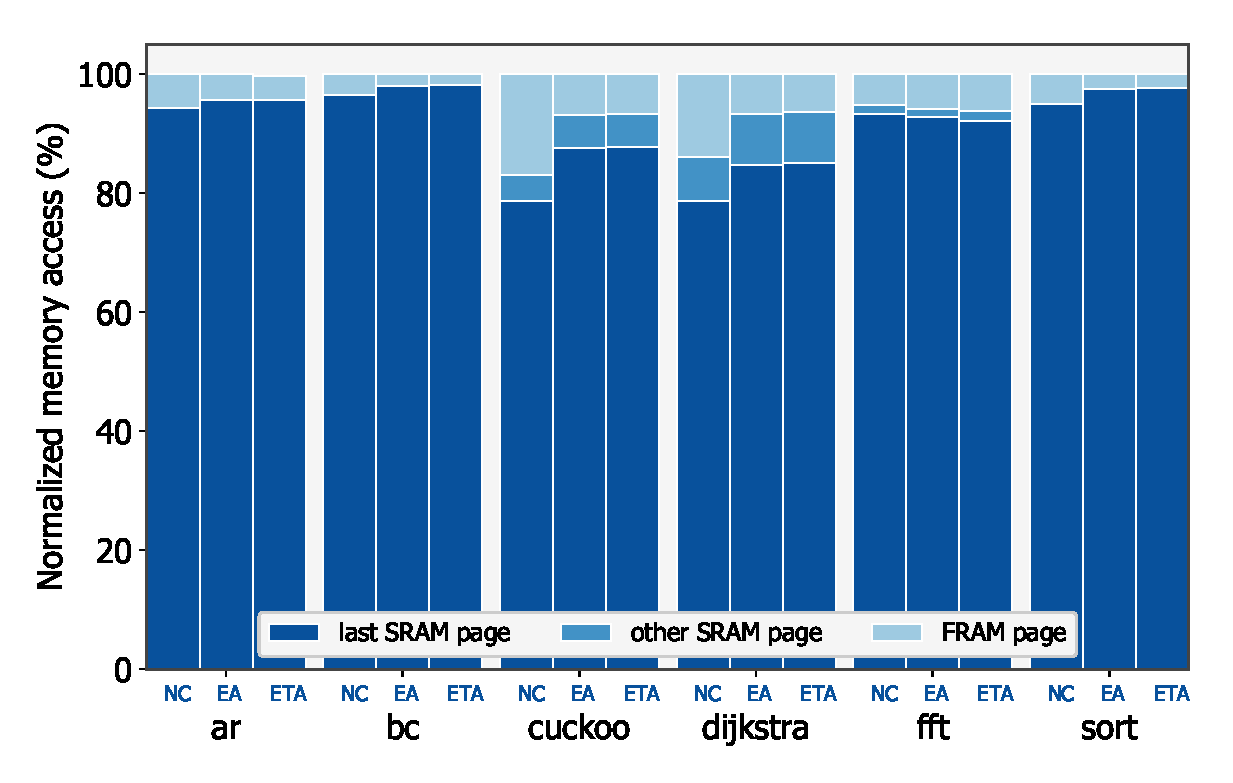
\includegraphics[width=0.49\columnwidth]{figures/memAccess}
	\caption{\sys kernel overhead. Left: high-level load distribution; right: detailed breakdown of memory accesses overhead (from the left figure). NC: no coalescing, EA: energy-aware coalescing, ETA: energy- and task-aware coalescing. \todo{rename legend entry 'task code' to 'user code'; rename y-axis to 'Load (\%)'}{Amjad}}
	\label{fig:coalEfficiency}
\end{figure}

\textbf{\sys Kernel Overhead Breakdown.} We now proceed with investigating how much utilization \sys's kernel steals to user code, quantifying task transitions and memory accesses overhead. For a broader picture, we profile kernel load for NC as well. The result for all benchmarks are measured in the same way as for the results presented above (i.e. given in Figure~\ref{fig:overallOverheadBreakdown}) and using the same page sizes as in the previous experiment. The outcome is presented in Figure~\ref{fig:coalEfficiency} (left side).
%
As expected, non-coalescing (NC) \sys introduces a huge cost of task transitions and commits (which recapitulates the result presented in Figure~\ref{fig:overallOverheadBreakdown}). For both coalescing strategies (EA and ETA) protected variables' accesses constitutes about 30\% of the whole load across all benchmarks. In fact, dynamic address translation is the most critical bottleneck for \sys.

\textbf{Protected Memory Accesses Breakdown.} Figure~\ref{fig:coalEfficiency} (right side) zooms into the overhead introduced by \sys's protected memory accesses.
% Let us now look into the results on the \sys memory operation process, i.e. we will show specifically which parts of memory from Figure~\ref{fig:coalEfficiency} (left) are accessed. The result is presented in Figure~\ref{fig:coalEfficiency} (right).
We immediately see that the majority of operations are targeting the most recently accessed SRAM page, and very few operations include a page swap from FRAM. There are very few cases involving SRAM pages other than the last one (only visible for \textbf{cuckoo} and \textbf{dijkstra}). This distinction is important because, when searching the \texttt{\underline{working}} buffer, the most recently accessed page is the first one being checked by \sys. This choice is highly motivated by this result. It is important to mention that memory access patterns are fully shaped by the application, and those ones which use a lot of protected memory can generate a higher rate of page swaps.

\subsection{Benchmark execution time}
\label{sec:result_coalescing}

\begin{wrapfigure}{t!}{0.5\textwidth}
%\begin{figure}
	\centering
	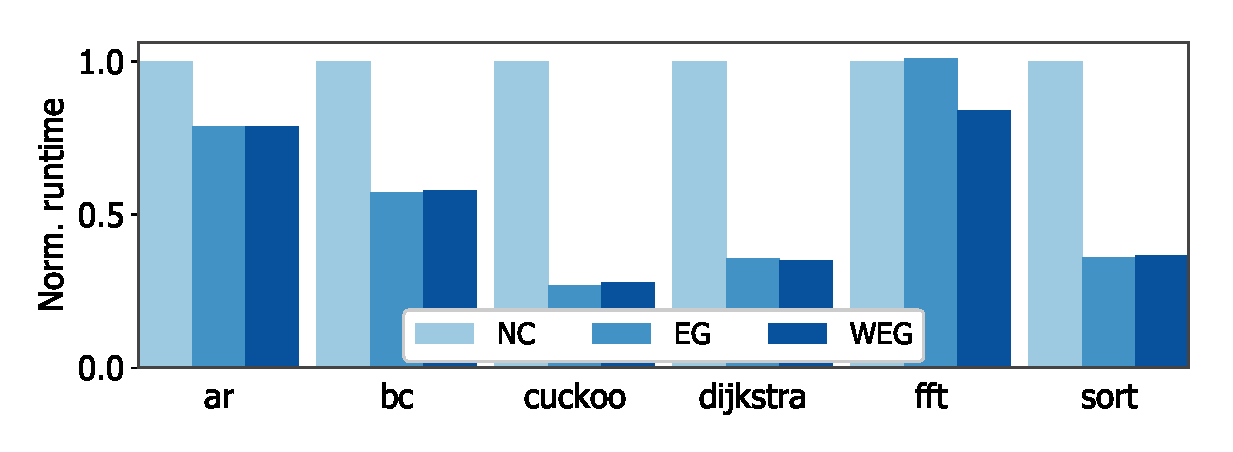
\includegraphics[width=0.5\columnwidth]{figures/coalStrategies}
	\caption{Coalescing strategies (EA and ETA) run time per application on intermittent power (RF generator at 15\,cm from the WISP), compared to \sys without coalescing (NC). Coalescing provides significant improvements: from 0.25 (\textbf{ar}) up to 0.70 (\textbf{sort}) compared to a non-coalescing system.}
	\label{fig:coalescing}
%\end{figure} 
\end{wrapfigure}

We proceed with characterizing \sys by studying how its execution time varies due to task adaptation. We look at \sys in isolation and in comparison to Alpaca.

\textbf{\sys Cross-Evaluation.} Figure~\ref{fig:coalescing} shows the run time of \sys's three coalescing strategies for all benchmarks normalized to NC's performances. We show data from experiments measured in the same way as for the results in Section~\ref{sec:coala_overhead}. 

The trend in Figure~\ref{fig:coalescing} recapitulates the result presented in Figure~\ref{fig:overallOverheadBreakdown} showing the benefit, in \emph {normalized runtime}, of coalescing (considering EA and ETA), for all applications. Coalescing improves performances by eliminating the overhead of committing after each task. The difference in performance between coalescing and no coalescing is, however, highly application-dependent. Then, the gain from the energy- and task-aware strategy (ETA) compared to energy-aware-only (EA) are almost non-existent for applications, except for \textbf{fft}. Actually, in some cases energy awareness solely introduces overhead. This behavior reflects an uniform task decomposition. When tasks have similar run time, it is pleonastic to count their load. As for \textbf{fft}, tasks are not so uniform, and this makes energy awareness necessary (for this benchmark, NC is better than EA).
Furthermore, benchmarks like \textbf{bc}, \textbf{cuckoo}, \textbf{dijkstra} and \textbf{sort} have small tasks that \sys can easily coalesce to eliminate many unnecessary commits.

\textbf{\sys versus non-adaptive Task-based Model.} We now evaluate \sys's run time and compare it to Alpaca---a non-adaptive task-based system. Results are presented in Figure~\ref{fig:runtime}. For each application we measured its execution time using real wireless power provisioned by the RF signal generator at three distances (refer again to Section~\ref{sec:implementation}). The plot presents the average execution time of each application for Coala and Alpaca, normalized to the latter. The results show that \sys provides a performance benefit compared to Alpaca for most applications (all except for \textbf{ar} and \textbf{cuckoo} at 30 and 50\,cm). The improvement is the greatest for applications that perform repeated write after read operations, particularly if involving arrays (\textbf{dijkstra}, \textbf{fft} and \textbf{sort}). This effect is seen at all distances on intermittent power. In applications with protected variables (or array elements) accessed next to each other, but residing in different SRAM or FRAM pages, \sys incurs overhead from memory virtualization that causes its performance to be comparable to (or worse than) Alpaca (\textbf{ar}, \textbf{cuckoo}).
%
Another critical observation is that \textbf{fft} benchmark did not complete at any distance larger than 0.15\,cm. As we will show now, \sys's task downscaling mechanism, which was intendedly disabled for this experiment, will be able to solve this issue.

\begin{wrapfigure}{t!}{0.5\textwidth}
%\begin{figure}
	\centering
	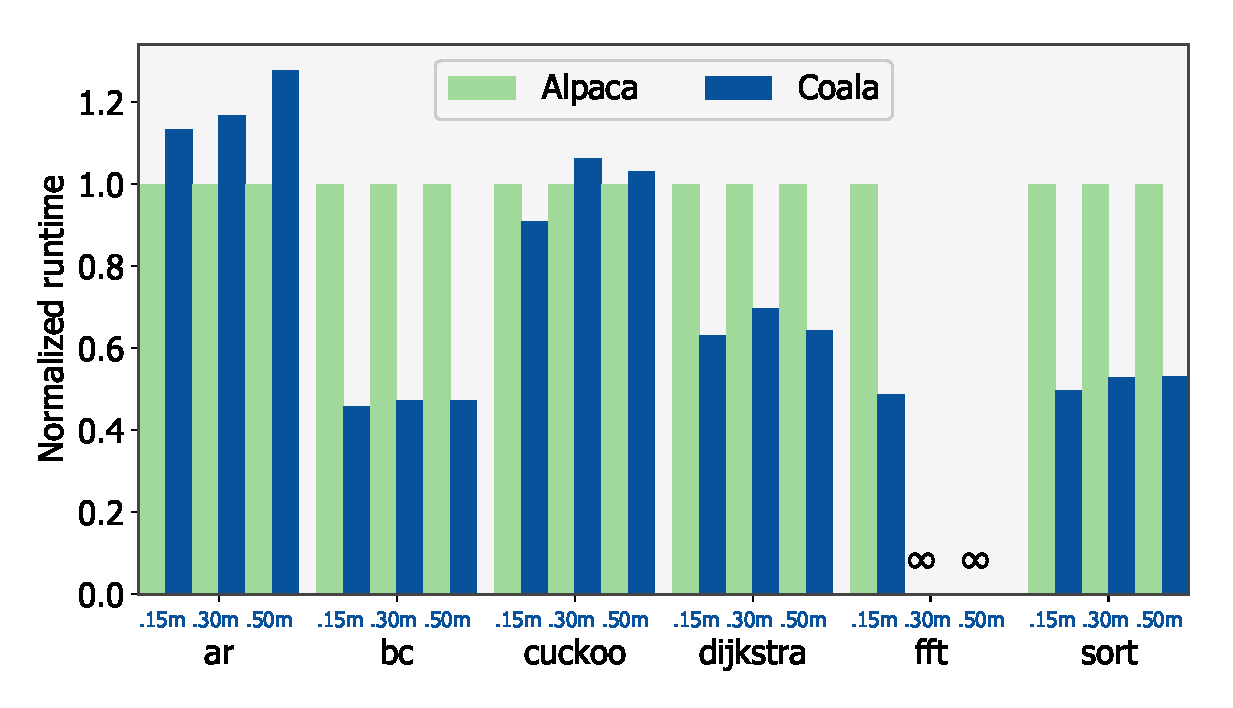
\includegraphics[width=0.5\columnwidth]{figures/coala_alpaca_gcc}
	\caption{Performance of \sys applications at multiple WISP to RF generator antenna distances \{0.15, 0.3, 0.5\}\,m (left, center and right-most bar per application, respectively), compared against Alpaca (results normalized) for ETA coalescing strategy. Results show that \sys performs on average better than Alpaca for majority of the benchmarks. For specific benchmarks \sys performs worse than Alpaca \todo{state why it is sometimes worse}{Carlo}}
	\label{fig:runtime}
%\end{figure}
\end{wrapfigure}

\textbf{Task Downscaling Execution Time.} We have enabled task downscaling and measured the execution time for \textbf{fft} benchmark at 60\,cm from the exciter, that is, even \emph{farther} than the farthest distance at which (without this feature) this benchmark could not run to completion (refer again to Figure~\ref{fig:coalescing} and $\infty$ marks). \sys could execute the benchmark successfully with an average `on' time (the time spent for useful computation excluding energy breaks) of 201\,ms for NC and of 180\,ms for ETA, respectively 2.16$\times$ and 2.31$\times$ slower than at 15\,cm, which is impressive compared to the infinite run time of Alpaca, being a static system.

\subsection{Paging Performance}
\label{sec:results_memory_management}

We have also evaluated the effect that paging with different page sizes has on \sys's performance, shown in Figure~\ref{fig:page_size}. The left-hand side plot shows the run time performance normalized to the best per-application performance, using pages of different sizes; the right-hand side plot shows the number of page faults for the same set of executions normalized to the minimum of each set. We measured performance as MCU clock cycles using values read out by TI's Code Composer Studio IDE. 

\textbf{Effect of Page Size on Run Time.} The results (Figure~\ref{fig:page_size}, left) show a ``bathtub curve'' in the performance of each application (the effect would be more profound with a larger set of pages than we considered), as the number of page faults varies. The data suggest that across applications there is a page size that minimizes execution time. We observe that the page size is not the same for each application, although 128\,B pages perform well for all applications. 

\textbf{Page Size versus Page Faults in \sys Runtime.} The increased rate of page faults (Figure~\ref{fig:page_size}, right) is responsible for the overhead with small page sizes; smaller pages require accessing more different pages, leading to higher paging costs. With larger page sizes, the overhead is higher than with moderate pages, too. The explanation for these higher overheads is that large pages have a higher commit cost. Even if an application accesses few memory locations, \sys pages data at full page size, degrading performance by sometimes paging in and out unnecessary data. The data reveal a reasonable default page size of 128\,B and, when developing an application, a programmer should consider varying the page size to moderate poor performance.

\begin{figure}
	\centering
	\includegraphics[width=0.49\columnwidth]{figures/page_exec-time}
	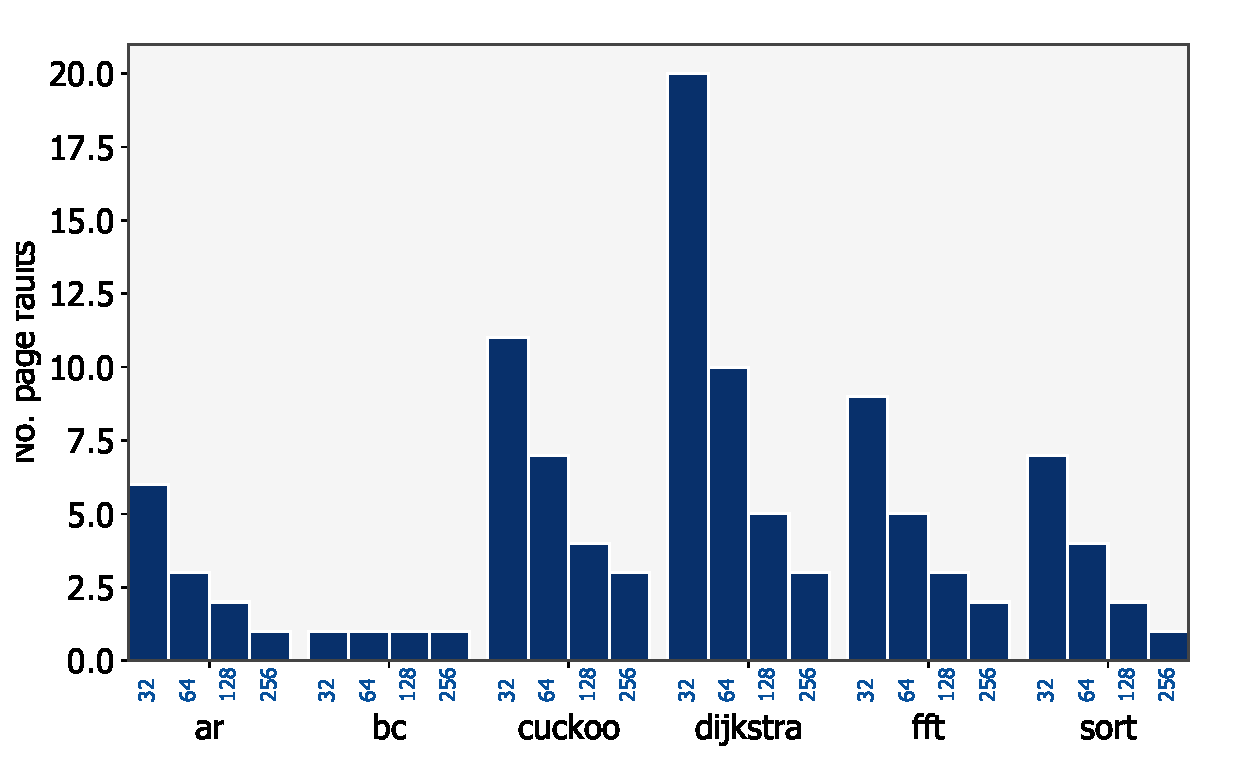
\includegraphics[width=0.49\columnwidth]{figures/pagePulls}
	\caption{\sys normalized runtime for various page sizes, \{32, 64,128,256\}\,B (left) and respective page pulls (bottom) for all benchmarks.}
	\label{fig:page_size}
\end{figure}

%\subsection{\sys Memory Footprint?}
%\label{sec:results_program_characterization}
%
%\begin{table}
%	\begin{tabular}{| c | c | c | c | c |}
%		\hline
%		\multirow{2}{*}{Application} & \multicolumn{2}{ c |}{Memory footprint} & \multirow{2}{*}{No. tasks} & \multirow{2}{*}{SLOC} \\
%		\cline{2-3}
%		{} & \sys & Alpaca & {} & {} \\
%		\hline\hline
%				\textbf{ar} & --- & --- & --- & ---\\
%		\hline
%				\textbf{bc} & --- & --- & --- & ---\\
%		\hline
%				\textbf{cuckoo} & --- & --- & --- & ---\\
%		\hline
%				\textbf{dijkstra} & --- & --- & --- & ---\\
%		\hline
%				\textbf{fft} & --- & --- & --- & ---\\
%		\hline
%				\textbf{sort} & --- & --- & --- & ---\\
%		\hline
%	\end{tabular}
%		\caption{Comparison between \sys and Alpaca benchmarks.}
%		\label{table:compiler_result}\vspace{-0.5cm}
%\end{table}

%\begin{table}[t]
%	\centering
%	\renewcommand{\tabcolsep}{1pt}
%	\begin{tabular}{|l|cc|cc|cc|cc|c|}
%		\hline
%		{} & \multicolumn{2}{c|}{{\bf Prot. bytes}} & \multicolumn{2}{c|}{{\bf \# Tasks}} & \multicolumn{2}{c|}{{\bf \# Prot. acc.}} & \multicolumn{2}{c|}{\bf SLOC} & {\bf Comp.} \\
%		App & Man. & Comp. & Man. & Comp. & Man. & Comp. & \multicolumn{1}{l}{\sys} & \multicolumn{1}{r|}{Chain~\cite{chain}} & {\bf time} \\
%		\hline\hline
%		bc & 22 & 22 & 10 & 15 & 81 & 93 & 351 &588 & 3\\
%		cem & 3492 & 3242 & 12 & 9 & 92 & 123 & 388 &721 & 2\\
%		cuckoo & 282 & 288 & 15 & 6 & 90 & 76 & 483 &762 & 6\\
%		rsa & 332 & 250 & 20 & 27 & 130 & 296 & 887 &1233 & 86\\
%		ar & 166 & 218 & 11 & 6 & 112 & 333 & 483 &762 & 34\\
%		sort & 104 & 104 & 4 & 2 & 70 & 23 & 180 & 287 & $<$1\\
%		dft$^\dagger$ & --- & --- & --- & --- & --- & --- & 222 & 293 & ---\\
%		%dd &  &  &  &  &  &  &  & 287 &  \\
%		\hline
%	\end{tabular}
%		\caption{Comparison between \sys and Alpaca benchmarks.}
%		\label{table:compiler_result}\vspace{-0.5cm}
%\end{table}
